\section{Wstęp}

\begin{frame}{Czym jest kryptografia asymetryczna}
    \begin{figure}
        \centering
            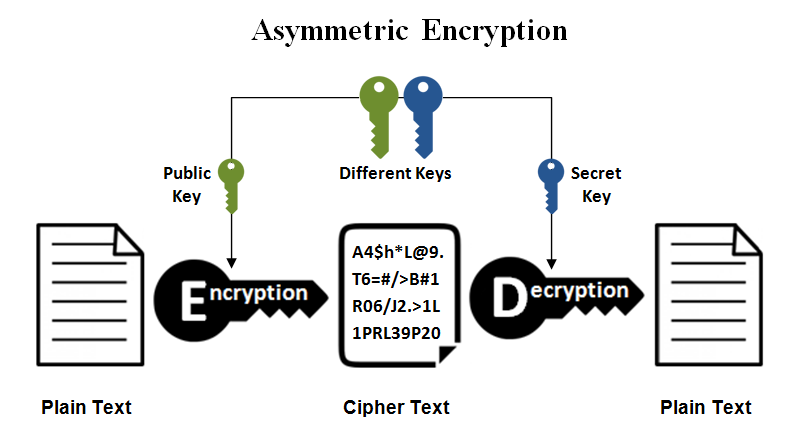
\includegraphics[height=0.45\textwidth]{introduction/graphics/Asymmetric-Encryption.png}
            \caption{Źródło: \cite{ssl2buy}}
    \end{figure}
\end{frame}

\begin{frame}{Jakie algortymy wybraliśmy}
    \begin{itemize}
        \item Puzle Merkle'a (1974)
        \item RSA (1977)
        \item ECC (1983)
    \end{itemize}

\end{frame}

\begin{frame}{Plan analizy porównawczej wybranych algorytmów}
    \begin{itemize}
        \item Podstawy matematyczne
        \pause
        \item Wykorzystanie w praktyce
        \pause
        \item Bezpieczeństwo teraz
        \pause
        \item Bezpieczeństwo w przyszłości
    \end{itemize}
\end{frame}